\section{关系模式及范式}
\begin{itemize}
    \item 关系模式由五部分组成,是一个五元组:$$R=(U,D,DOM,F)$$
    \begin{itemize}
        \item 关系名 $R$ 是符号化的元组语义
        \item $U$ 为一组属性
        \item $D$ 为属性组 $U$ 中的属性所来自的域
        \item $DOM$ 为属性到域的映射
        \item $F$ 为属性组 $U$ 上的一组数据依赖
    \end{itemize}
    \item 由于 $D$、$DOM$ 与模式设计关系不大,因此可以把关系模式看作一个三元组:$R\langle U,F\rangle$
    \begin{itemize}
        \item 当且仅当 $U$ 上的一个关系 $r$ 满足 $F$ 时,$r$ 称为关系模式 $R\langle U,F\rangle$ 的一个关系
        \item 作为二维表,关系要符合一个最基本的条件:每个分量必须是不可分开的数据项。满足了这个条件的关系模式就属于\textbf{第一范式}(1NF)
    \end{itemize}
    \item 数据依赖
    \begin{itemize}
        \item 是一个关系内部属性与属性之间的一种约束关系
        \begin{itemize}
            \item 通过属性间值的相等与否体现出来的数据间相关联系
        \end{itemize}
    \end{itemize}
    \item 是现实世界属性间相互联系的抽象
    \begin{itemize}
        \item 是数据内在的性质
    \end{itemize}
    \item 是语义的体现
    \item 数据依赖的主要类型
    \begin{itemize}
        \item 函数依赖(Functional Dependency,简记为 FD)
        \item 多值依赖(Multi-Valued Dependency,简记为 MVD)
    \end{itemize}
    \item 第一范式的问题有
    \vspace{-0.8em}
	\begin{multicols}{4}
        \begin{itemize}
            \item 数据冗余
            \item 更新异常
            \item 插入异常
            \item 删除异常
        \end{itemize}
	\end{multicols}
	\vspace{-1em}
\end{itemize}

\section{规范化}

\subsection{函数依赖}
设 $R(U)$ 是一个属性集 $U$ 上的关系模式,$X$ 和 $Y$ 是 $U$ 的子集。若对于 $R(U)$ 的任意一个可能的关系 $r$,$r$ 中不可能存在两个元组在 $X$ 上的属性值相等,而在 $Y$ 上的属性值不等, 则称“$X$ 函数确定 $Y$”或“$Y$ 函数依赖于 $X$”,记作 $X\to Y$,$X$ 称为这个函数依赖的决定因素
\begin{itemize}
    \item 函数依赖不是指关系模式 $R$ 的某个或某些关系实例满足的约束条件,而是指 $R$ 的所有关系实例均要满足的约束条件
    \item 函数依赖是语义范畴的概念。只能根据数据的语义来确定函数依赖
    \item 数据库设计者可以对现实世界作强制的规定
\end{itemize}

在关系模式 $R(U)$ 中,对于 $U$ 的子集 $X$ 和 $Y$,
\begin{itemize}
    \item $X\to Y$,但 $Y\not\subseteq X$,则称 $X \to Y$ 是非平凡的函数依赖
    \item $X\to Y$,但 $Y\subseteq X$,则称 $X \to Y$ 是平凡的函数依赖
    \item 对于任一关系模式,平凡函数依赖都是必然成立的,它不反映新的语义。因此若不特别声明,我们总是讨论非平凡函数依赖
\end{itemize}

在 $R(U)$ 中,如果 $X \to Y$,并且对于 $X$ 的任何一个真子集 $X ^\prime$,都有 $X^\prime \nrightarrow  Y$, 则称 $Y$ 对 $X$ 完全函数依赖,记作 $X \stackrel{F}{\longrightarrow} Y$
\begin{itemize}
    \item 若 $X \to Y$,但 $Y$ 不完全函数依赖于 $X$,则称 $Y$ 对 $X$ 部分函数依赖,记作 $X \stackrel{P}{\longrightarrow} Y$
\end{itemize}

在 $R(U)$ 中,如果 $X \to Y(Y\not\subseteq X )$,$Y \nrightarrow  X$,$Y\to Z$,$Z\not\subseteq Y$, 则称 $Z$ 对 $X$ 传递函数依赖,记为:$X\stackrel{\mbox{传递}}{\longrightarrow} Z$
\begin{itemize}
    \item 如果 $Y\to X$, 即 $X\leftarrow \to Y$,则 $Z$ 直接依赖于 $X$,而不是传递函数依赖
\end{itemize}

\subsection{码}
设 $K$ 为$R\langle U,F\rangle$中的属性或属性组合。若 $K \stackrel{F}{\longrightarrow} U$,则 $K$ 称为 $R$ 的一个候选码
\begin{itemize}
    \item 如果 $U$ 部分函数依赖于 $K$,即 $K \stackrel{P}{\longrightarrow} U$,则 $K$ 称为超码
    \begin{itemize}
        \item 候选码的超集是超码,候选码的真子集一定不是超码
    \end{itemize}
    \item 若关系模式 $R$ 有多个候选码,则选定其中的一个做为主码
    \item 主属性与非主属性
    \begin{itemize}
        \item 包含在任何一个候选码中的属性 ,称为主属性
        \item 不包含在任何码中的属性称为非主属性或非码属性
    \end{itemize}
    \item 全码:整个属性组是码,称为全码
\end{itemize}

关系模式 $R$ 中属性或属性组 $X$ 并非 $R$ 的码,但 $X$ 是另一个关系模式的码,则称 $X$ 是 $R$ 的外部码也称外码

主码与外部码一起提供了表示关系间联系的手段

\subsection{范式}
\begin{itemize}
    \item 范式是符合某一种级别的关系模式的集合
    \item 关系数据库中的关系必须满足一定的要求。满足不同程度要求的为不同范式
    \item 一个低一级范式的关系模式,通过模式分解可以转换为若干个高一级范式的关系模式的集合,这种过程就叫规范化
\end{itemize}

\begin{figure}[H]
    \vspace{-0.5em}
	\centering
	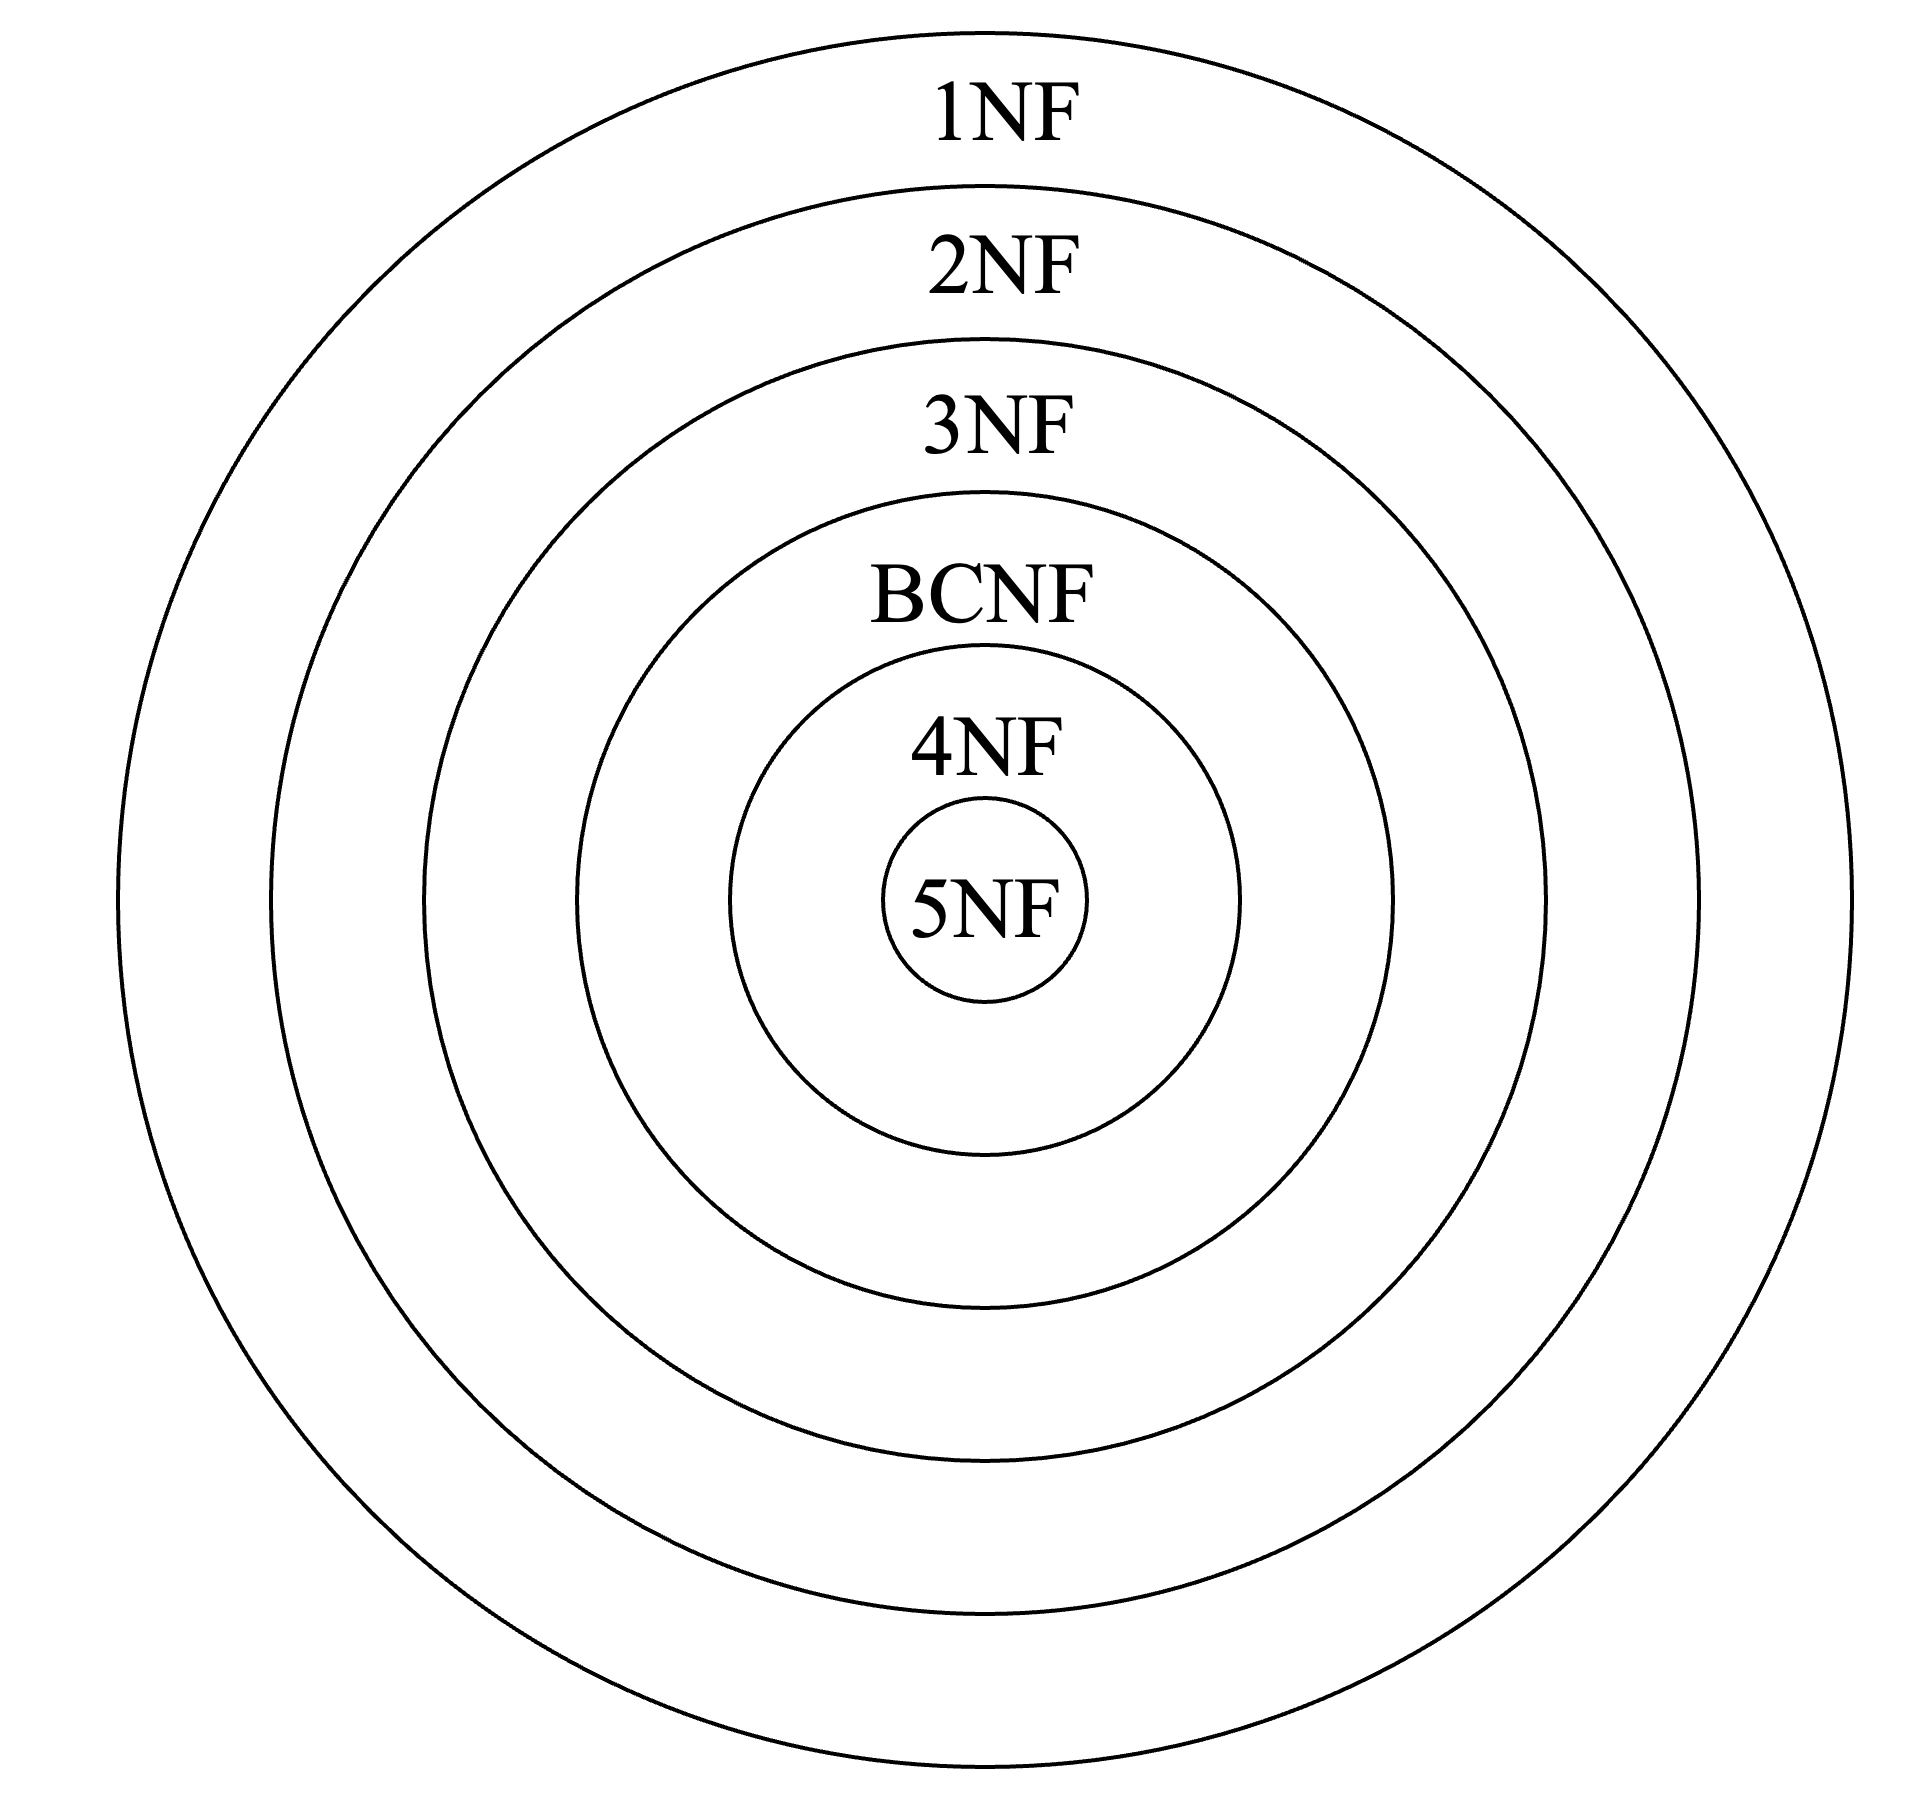
\includegraphics[width=0.4\textwidth]{images/6.2.3}
    \vspace{-1em}
\end{figure}

\subsection{2NF}
若关系模式 $R\in 1\mathrm{NF}$,并且每一个非主属性都完全函数依赖于任何一个候选码,则 $R\in 2\mathrm{NF}$

\subsection{3NF}
设关系模式 $R\langle U,F\rangle \in 1\mathrm{NF}$,若 $R$ 中不存在这样的码 $X$、属性组 $Y$ 及非主属性 $Z(Z\not \subseteq Y)$,使得 $X\to Y$,$Y\to Z$ 成立,$Y \nrightarrow  X$ 不成立,则称 $R\langle U,F\rangle \in 3\mathrm{NF}$

\subsection{BCNF}
\begin{itemize}
    \item BCNF 由 Boyce 和 Codd 提出,比 3NF更进了一步。通常认为 BCNF 是修正的第三范式,有时也称为扩充的第三范式
    \item 设关系模式 $R\langle U,F\rangle \in 1\mathrm{NF}$,若 $X\to Y$ 且 $Y\not \subseteq X$时 $X$ 必含有码,则 $R\langle U,F\rangle \in \mathrm{BCNF}$
    \item 换言之,在关系模式 $R\langle U,F\rangle$ 中,如果每一个决定属性集都包含候选码,则 $R\in \mathrm{BCNF}$
    \item BCNF 的关系模式所具有的性质
    \begin{itemize}
        \item 所有非主属性都完全函数依赖于每个候选码
        \item 所有主属性都完全函数依赖于每个不包含它的候选码
        \item 没有任何属性完全函数依赖于非码的任何一组属性
    \end{itemize}
    \item 如果一个关系数据库中的所有关系模式都属于 BCNF,那么在函数依赖范畴内,它已实现了模式的彻底分解,达到了最高的规范化程度,消除了插入异常和删除异常
\end{itemize}

\subsection{多值依赖}
设 $R(U)$ 是属性集 $U$ 上的一个关系模式。$X,Y,Z$ 是 $U$ 的子集,并且 $Z=U-X-Y$。关系模式 $R(U)$ 中多值依赖 $X\to \to Y$ 成立,当且仅当对 $R(U)$ 的任一关系 $r$,给定的一对 $(x,z)$ 值,有一组 $Y$ 的值,这组值仅仅决定于 $x$ 值而与 $z$ 值无关
\begin{itemize}
    \item 平凡多值依赖和非平凡的多值依赖
    \begin{itemize}
        \item 若 $X\to \to Y$,而 $Z = \emptyset$,即 $Z$ 为空,则称 $X\to \to Y$ 为平凡的多值依赖
        \item 否则称 $X\to \to Y$ 为非平凡的多值依赖
    \end{itemize}
\end{itemize}

多值依赖的另一个等价的定义:在 $R(U)$ 的任一关系 $r$ 中,如果存在元组 $t,s$ 使得 $t[X] = s[X]$,那么就必然存在元组 $w,v \in r$,($w,v$ 可以与 $s,t$ 相同),使得 $w[X] = v[X] = t[X]$,而 $W[Y] = t[Y],w[Z] = s[Z],v[Y]=s[Y],v[Z]=t[Z]$(即交换 $s,t$ 元组的 $Y$ 值所得的两个新元组必在 $r$ 中,则 $Y$ 多值依赖于 $X$,记为 $X\to\to Y$。这里 $X,Y$ 是 $U$ 的子集,$Z = U-X-Y$

多值依赖的性质:
\begin{itemize}
    \item 多值依赖具有对称性。即若 $X\to\to Y$,则 $X\to\to Z$,其中 $Z=U-X-Y$
    \item 多值依赖具有传递性。即若 $X\to\to Y$,$Y\to\to Z$, 则 $X\to\to Z-Y$
    \item 函数依赖是多值依赖的特殊情况。即若 $X\to Y$,则 $X\to \to Y$
    \item 若 $X\to\to Y$,$X\to\to Z$,则 $X\to \to YZ$
    \item 若 $X\to\to Y$,$X\to\to Z$,则 $X\to \to Y \cap Z$
    \item 若 $X\to\to Y$,$X\to\to Z$,则 $X\to \to Y-Z,X\to \to Z-Y$
\end{itemize}

多值依赖与函数依赖的区别
\begin{itemize}
    \item 多值依赖的有效性与属性集的范围有关,函数依赖$X\to Y$的有效性仅决定于$X$、$Y$这两个属性集的值
    \begin{itemize}
        \item 若 $X\to\to Y$ 在 $U$上成立,则在 $W(XY \subseteq W \subseteq U)$ 上一定成立;反之则不然,即 $X\to\to Y$ 在 $W(W\subset U)$上成立,在 $U$ 上并不一定成立。
        \item 原因:多值依赖的定义中不仅涉及属性组 $X$ 和 $Y$,而且涉及 $U$ 中其余属性 $Z$  
        \item 一般地,在 $R(U)$ 上若有 $X\to\to Y$ 在 $W(W\subset U)$ 上成立,则称 $X\to\to Y$ 为 $R(U)$ 的嵌入型多值依赖
    \end{itemize}
    \item 若函数依赖 $X\to\to Y$ 在 $R(U)$ 上成立,则对于任何 $Y^\prime \subset Y$ 均有 $X\to Y^\prime$ 成立。多值依赖 $X\to\to Y$若在 $R(U)$ 上成立,不能断言对于任何 $Y^\prime Y$ 有 $X\to \to Y^\prime$ 成立
\end{itemize}

\subsection{4NF}
关系模式 $R\langle U,F\rangle \in 1\mathrm{NF}$,如果对于R的每个非平凡多值依赖$X\to \to Y(Y \not \subseteq X)$,$X$ 都含有码,则 $R\langle U,F\rangle \in 4\mathrm{NF}$

4NF 就是限制关系模式的属性之间不允许有非平凡且非函数依赖的多值依赖。4NF 所允许的非平凡多值依赖实际上是函数依赖